% !TEX root = ../../semexp-thesis.tex

\section{A Blackboard Framework for Managing Suggestions}
\label{sec:design/suggestions}

When the suggestion engine is invoked, it first captures the implicit context of programmers as \emph{artifacts}---for example, currently viewed methods, recent experiments, or notes.
It then executes different \emph{strategies} to suggest further artifacts based on the former.
For example, given a currently viewed method, different strategies could suggest senders of this method, similar methods, or related documentation artifacts.
To anticipate larger parts of the programmer's research process, suggestions are not limited to initial input artifacts but can also be derived from prior suggestions.
In our example, a fourth strategy could extract and suggest popular message sends from similar methods.

These requirements create a high complexity in the suggestion engine, which has to manage different types of artifacts, strategies, and a convoluted dataflow.
To handle this complexity and maintain flexibility in the design of new artifacts and strategies, we define a \emph{blackboard framework} that organizes artifacts and orchestrates strategies.

\begin{figure}
	\centering
	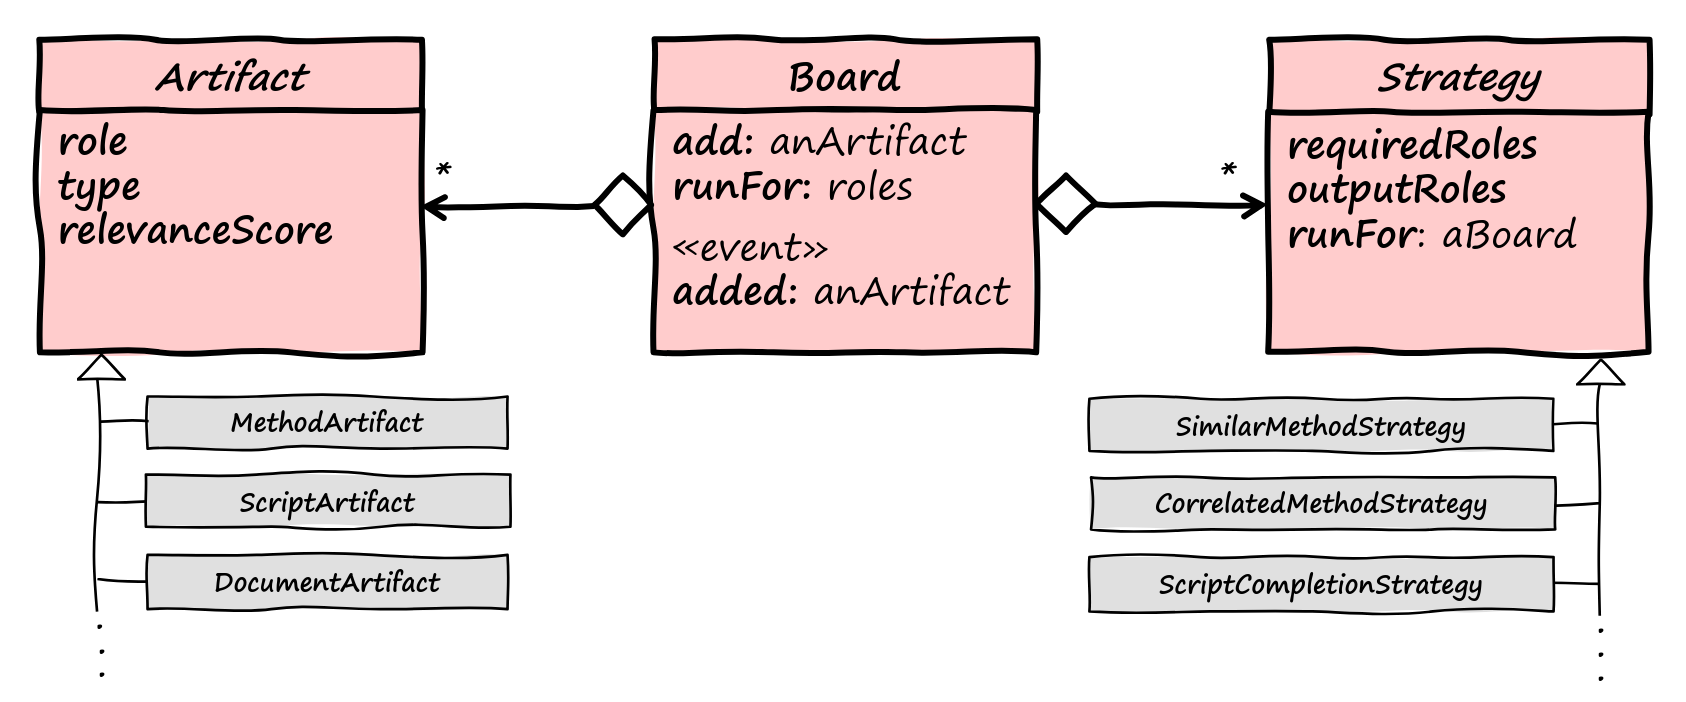
\includegraphics[width=\textwidth]{02_suggestions/classes.png}
	\caption[The general object model of our \emph{blackboard framework} for creating suggestions.]{
		The general object model of our blackboard framework for creating suggestions (UML class diagram with Smalltalk-styled method signatures).
		A central \emph{board} maintains many \emph{artifacts} of different types and roles, and it has access to \emph{strategies} that consume existing artifacts to produce new artifacts.
		When asked for suggestion artifacts of certain roles, the board identifies and schedules all required strategies and returns the new suggestions to the requestor.
	}
	\label{fig:design/suggestions/classes}
\end{figure}

The framework defines a central board, on which different artifacts can be arranged.
Each artifact is specified with a \emph{role} (such as input artifact, similar artifact, or method sender) and a \emph{type} (such as class, method, or documentation).
Additionally, the board contains a set of strategies, each of which is able to consume given artifacts and produce more artifacts.
Each strategy can specify a set of \emph{required roles} for the artifacts it consumes as well as a set of \emph{output roles} for the artifacts it produces.
\Cref{fig:design/suggestions/classes} displays our object model of the blackboard framework.

After the board has been configured with a concrete set of input artifacts and strategies, it can be invoked to provide suggestions of certain roles.
Once invoked, the board determines all available strategies that can produce the requested artifact roles and schedules them.
If any strategy defines requirements, the board first checks whether they are met by the current set of artifacts, or otherwise attempts to determine and schedule further strategies that produce artifacts of the required role.
This process continues recursively until all possible strategies that are directly or indirectly required to fulfill the request have been scheduled.
All scheduled strategies are executed concurrently as soon as their requirements have been resolved, and each running strategy adds new artifacts to the board.
Finally, the requestor can access or stream the resulting artifacts from the board.

The board framework also provides strategies for organizing artifacts:
for example, identical or equivalent artifacts that have been produced by multiple strategies can be merged, artifacts can be grouped based on their role, type, or metadata, and they can be sorted based on ranks provided by prior strategies.

To support debugging and observability, strategies can also be executed synchronously, and a provenance mechanism\textlabel{idx:design/suggestions/provenance} remembers the original strategy and its input artifacts for every produced artifact.

\begin{example}
	A programmer has drafted a new method and a short list of to-do notes in their programming system.
	To provide them with further possibly relevant message sends for their method draft, the semantic workspace invokes the suggestion engine with both artifacts and requests suggestions of the role ``correlated message''~(\cref{fig:design/suggestions/example}).

	Once invoked, the suggestion engine identifies two strategies that can suggest correlated messages: a \emph{correlated selectors} strategy and a \emph{method harvester} strategy~(see \cpageref{sec:suggestions/search/correlations}).
	Both strategies require artifacts of the role ``similar method'', which are currently not present on the board.
	For this reason, the suggestion engine finds two other strategies that can produce similar method artifacts: a \emph{semantic method search} strategy and a \emph{TF-IDF selector search} strategy.
	Both these search strategies require artifacts of the role ``input'', thus their requirements are met and the engine schedules them.

	\vspace{\baselineskip}
	\begin{center}
		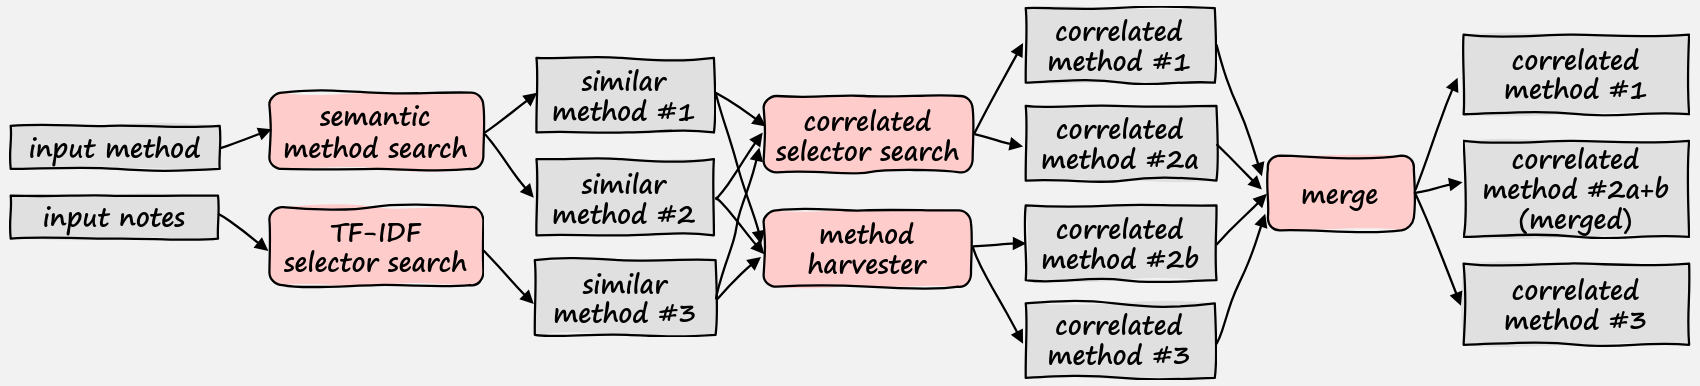
\includegraphics[width=\textwidth]{02_suggestions/example.png}
		\captionof{figure}[The involved artifacts and scheduled strategies for invoking the blackboard framework to find correlated methods for a given input method and notes.]{
			The involved artifacts and scheduled strategies for invoking the blackboard framework with our example.
		}
		\label{fig:design/suggestions/example}
	\end{center}

	Once the search strategies have finished and placed similar method artifacts on the board, the engine also executes the correlating strategies, leading to the addition of correlated messages and correlated methods to the board.
	The suggestion engine now merges both artifact types by attempting to associate all method artifacts with the same method name with a corresponding correlated message artifact.
	Finally, the resulting artifacts are ranked based on the original similarity scores and the correlation scores.
\end{example}

Thus, our blackboard framework shares characteristics from two existing approaches: \emph{blackboard systems} and \emph{data orchestration pipelines}.
First, it resembles the \emph{blackboard architecture pattern}~\cite[p.~71ff.]{buschmann1996pattern} and \emph{blackboard systems} from early expert systems~\cite{hayes1985blackboard}, where different \emph{knowledge sources} successively populate a \emph{blackboard} orchestrated by a \emph{control shell}.
Second, it is related to \emph{data orchestration pipelines}, which model and execute a directed acyclic graph of \emph{tasks}~\cite{talia2013workflow}.

However, our blackboard framework follows a more structured approach than traditional blackboard systems in that all strategies define static output roles, allowing to predict the dataflow in advance and schedule strategies in a top-down manner (as opposed to the bottom-up method of blackboard systems).
At the same time, the blackboard framework offers greater flexibility than data orchestration pipelines, which typically model direct dependencies between tasks rather than data roles, and thus allows for the implicit choice and combination of different strategies.
